\documentclass[12pt, a4paper]{article}

% ---- Paquetes ----
\usepackage[utf8]{inputenc}
\usepackage[spanish]{babel}
\usepackage[T1]{fontenc}
\usepackage{geometry}
\usepackage{graphicx}
\usepackage{enumitem}
\usepackage{xcolor}
\usepackage{fancyhdr}
\usepackage{hyperref}
\usepackage{listings}
\usepackage{amsmath}
\usepackage{booktabs}

% ---- Geomtría ----
\geometry{
    left=2.5cm,
    right=2.5cm,
    top=3cm,
    bottom=3cm
}

% ---- Hipervínculos ----
\hypersetup{
    colorlinks=true,
    linkcolor=blue!60!black,
    urlcolor=blue!60!black,
    citecolor=blue!60!black
}

% ---- Encabezado / Pie de página ----
\pagestyle{fancy}
\fancyhf{}
\fancyhead[L]{Fundamentos de Bases de Datos}
\fancyhead[R]{Tema 4 -- Normalización}
\fancyfoot[C]{\thepage}
\renewcommand{\headrulewidth}{0.4pt}
\renewcommand{\footrulewidth}{0.4pt}

% ---- Portada ----
\newcommand{\makeportada}{%
    \begin{titlepage}
        \centering

        \vspace*{0.5cm}



        \vspace{1cm}

        {\large \textsc{Instituto Tecnológico de Orizaba}\par}

        \vspace{0.3cm}

        {\large \textsc{Tecnológico Nacional de México}\par}

        \vspace{1.5cm}

        \rule{\textwidth}{1.5pt}

        \vspace{0.5cm}

        {\Huge \textbf{Tema 4 -- Normalización}\par}

        \vspace{0.4cm}

        {\LARGE Tarea 3 -- Formas Normales 1 a 5\\desde diagrama de clases\par}

        \vspace{0.5cm}

        \rule{\textwidth}{1.5pt}

        \vspace{1.5cm}

        {\large \textbf{Materia:} Fundamentos de Bases de Datos\par}

        \vspace{0.3cm}

        {\large \textbf{Grupo:} 4g3D\par}

        \vspace{0.6cm}

        {\large \textbf{Alumno:} Ricoy Aguirre Mayahua\par}

        \vspace{0.3cm}

        {\large \textbf{Carrera:} Ingeniería en Sistemas Computacionales\par}

        \vspace{0.3cm}

        {\large \textbf{Fecha:} \today\par}

        \vspace{2cm}

        \begin{flushright}
            \textit{``La normalización no es un lujo,\\ es la base de un modelo sólido.''}
        \end{flushright}

        \vfill
    \end{titlepage}
}

% ---- Estilo código SQL ----
\lstdefinestyle{sql}{
    language=SQL,
    basicstyle=\ttfamily\small,
    keywordstyle=\color{blue!70!black}\bfseries,
    commentstyle=\color{gray},
    stringstyle=\color{orange},
    numbers=left,
    numberstyle=\tiny\color{gray},
    stepnumber=1,
    numbersep=8pt,
    showstringspaces=false,
    breaklines=true,
    frame=single,
    tabsize=4,
    captionpos=b
}

% ---- Inicio del documento ----
\begin{document}

% ---- Portada ----
\makeportada

% ---- Índice ----
\tableofcontents
\newpage

% ---- Resumen / Introducción ----
\section{Introducción}

El presente documento describe el proceso de normalización de un modelo de base de datos aplicando las cinco formas normales (1FN a 5FN), partiendo de un diagrama de clases previamente diseñado. El objetivo es garantizar la integridad, consistencia y ausencia de redundancias en el esquema relacional, asegurando que cada tabla represente una única entidad del dominio del problema.

\section{Diagrama Entidad-Relación}

Este diagrama fue realizado con el propósito de tener una idea clara de las primeras 3 formas normales, ya que, como se describió en clase, al realizar este tipo de diagramas se puede obtener con mayor claridad una base de datos en 3\textsuperscript{a} Forma Normal.

\begin{figure}[ht]
    \centering
    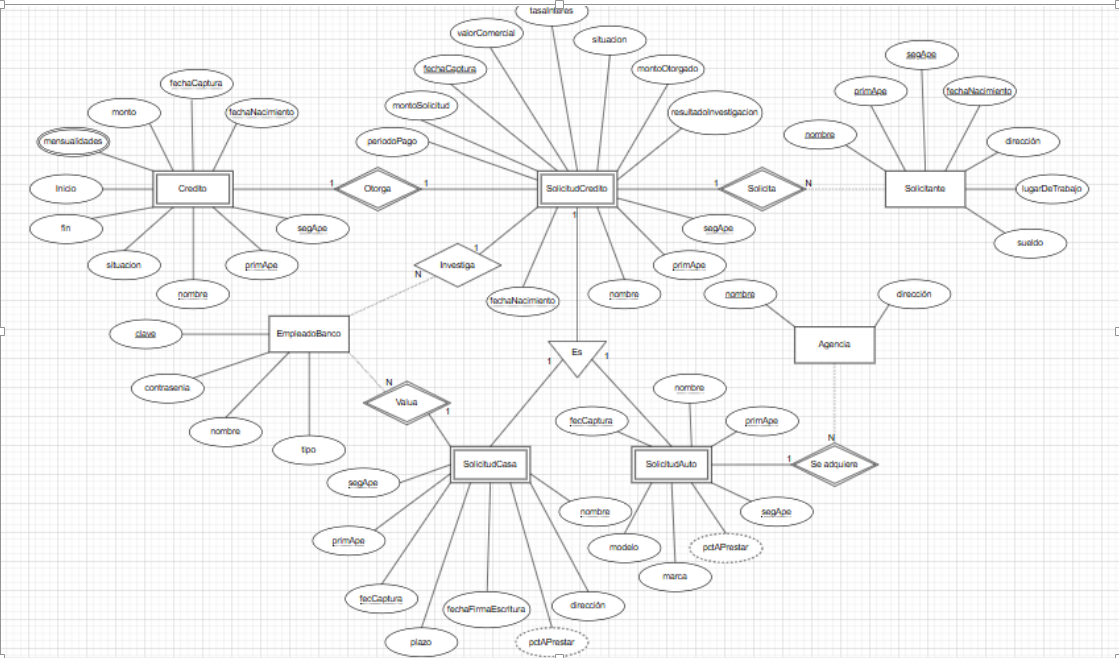
\includegraphics[width=\textwidth, keepaspectratio]{image.png}
    \caption{Diagrama Entidad-Relación del modelo de solicitudes de crédito.}
    \label{fig:er-diagram}
\end{figure}

\section{Base de Datos antes de las Formas Normales}

A continuación se presenta el conjunto inicial de tablas con sus respectivos atributos y referencias.

\subsection*{Relaciones Iniciales}

\begin{itemize}[leftmargin=2cm, label={--}]
    \item \textbf{Solicitante} (nombre, primApe, segApe, fechaNacimiento, dirección, lugarDeTrabajo, sueldo)
    \item \textbf{SolicitudCrédito} (fechaCaptura, nombre (FK), primApe (FK), segApe (FK), fechaNacimiento (FK), valorComercial, montoSolicitado, situacion, montoOtorgado, periodoPago, investigadorAsignado (FK), tasaInteres, resultadoInvestigacion)
    \item \textbf{Credito} (fechaCaptura (FK), nombre (FK), primApe (FK), segApe (FK), fechaNacimiento (FK), inicio, monto, fin, situación, mensualidades)
    \item \textbf{EmpleadoBanco} (clave, contrasenia, nombre, tipo)
    \item \textbf{SolicitudCasa} (fechaCaptura (FK), nombre (FK), primApe (FK), segApe (FK), fechaNacimiento (FK), fechaFirmaEscritura, plazo, dirección, pctAPrestar, valuadorAsignado (FK))
    \item \textbf{SolicitudAuto} (fecCaptura (FK), nombre (FK), primApe (FK), segApe (FK), fechaNacimiento (FK), marca, modelo, plazo, agencia)
    \item \textbf{Agencia} (nombre, dirección)
\end{itemize}

\newpage

\section{Primera Forma Normal (1FN)}

\textbf{Definición:} Una tabla está en 1FN si los dominios de todos sus atributos son atómicos; es decir, si no es necesario acceder a las partes.

\subsection*{Aplicación}

Para cumplir con esta forma normal, se requiere que las mensualidades dejen de ser un conjunto o arreglo de valores, transformándolo en su propia tabla. El resto de las relaciones permanecen sin cambios.

\subsection*{Esquema Resultante}

\begin{itemize}[leftmargin=2cm, label={--}]
    \item \textbf{Solicitante} (nombre, primApe, segApe, fechaNacimiento, dirección, lugarDeTrabajo, sueldo)
    \item \textbf{SolicitudCrédito} (fechaCaptura, nombre (FK), primApe (FK), segApe (FK), fechaNacimiento (FK), valorComercial, montoSolicitado, situacion, montoOtorgado, periodoPago, investigadorAsignado, tasaInteres, resultadoInvestigacion)
    \item \textbf{Credito} (fechaCaptura (FK), nombre (FK), primApe (FK), segApe (FK), fechaNacimiento (FK), inicio, monto, fin, situación)
    \item \textbf{Mensualidad} (fechaCaptura (FK), nombre (FK), primApe (FK), segApe (FK), fechaNacimiento (FK), numMensualidad, montoMensualidad)
    \item \textbf{EmpleadoBanco} (clave, contrasenia, nombre, tipo)
    \item \textbf{SolicitudCasa} (fechaCaptura (FK), nombre (FK), primApe (FK), segApe (FK), fechaNacimiento (FK), fechaFirmaEscritura, plazo, dirección, pctAPrestar)
    \item \textbf{SolicitudAuto} (fecCaptura (FK), nombre (FK), primApe (FK), segApe (FK), fechaNacimiento (FK), marca, modelo, plazo, agencia)
    \item \textbf{Agencia} (nombre, dirección)
\end{itemize}

\section{Segunda Forma Normal (2FN)}

\textbf{Definición:} Una tabla está en 2FN si, además de estar en 1FN, todas las columnas que \textbf{no} forman parte de una clave candidata sólo suministran información de la clave completa.

\subsection*{Aplicación}

En este caso se mantienen las formas de 1FN, ya que los atributos dependen de la llave única (como en \texttt{Agencia} o \texttt{EmpleadoBanco}), al igual que en otros casos se basan en la composición de todas las partes de la llave primaria (como en \texttt{SolicitudCrédito} o sus derivadas).

\noindent
\fcolorbox{blue!30}{blue!10}{%
    \parbox{\dimexpr\textwidth-2\fboxsep-2\fboxrule\relax}{%
        \textbf{Conclusión:} No se realiza ningún cambio al modelo.
    }%
}

\section{Tercera Forma Normal (3FN)}

\textbf{Definición:} Una relación está en tercera forma normal (3FN) si y sólo si está en 2FN y, además, todas las columnas que no sean claves dependen de la clave completa de forma no transitiva.

\subsection*{Aplicación}

En este caso, lo único que se hará es señalar que \texttt{montoOtorgado} es un atributo derivado, esto debido a que resulta de la operación:

\[
\text{montoOtorgado} = \text{valorComercial} \times \text{pctAPrestar}
\]

Por lo cual se deriva más a un método que a un atributo en sí, aunque lo tomaremos como un campo calculado no almacenable de forma redundante. Igualmente, este es un atributo relevante para el propósito de la solicitud.

\vspace{0.3cm}
\noindent
\fcolorbox{blue!30}{blue!10}{%
    \parbox{\dimexpr\textwidth-2\fboxsep-2\fboxrule\relax}{%
        \textbf{Conclusión:} Nuestro modelo relacional no se afecta; solo se dispone de una nota como restricción de dominio.
    }%
}

\newpage

\section{Forma Normal Boyce-Codd (FNBC)}

\textbf{Definición:} Es más estricta que la 3FN; se presenta cuando existen llaves compuestas. Elimina absolutamente todas las redundancias basadas en dependencias funcionales.

\subsection*{Aplicación}

En este aspecto, el haber decidido crear tablas para los padres e hijos desde el comienzo de nuestro modelo facilitó que en este punto no tengamos que dividir una tabla enorme como \texttt{SolicitudCrédito}, ya que cada una de las entidades hijas tiene especificados los atributos que posee y, por ende, no existe ninguna dependencia funcional.

\vspace{0.3cm}
\noindent
\fcolorbox{blue!30}{blue!10}{%
    \parbox{\dimexpr\textwidth-2\fboxsep-2\fboxrule\relax}{%
        \textbf{Conclusión:} Nuestro modelo no presenta ningún problema con respecto a FNBC, por lo que avanzamos a la siguiente forma.
    }%
}

\section{Cuarta Forma Normal (4FN)}

\textbf{Definición:} Una relación está en cuarta forma normal (4FN) si y sólo si está en 3FN y además no existen dependencias multivaloradas.

\subsection*{Aplicación}

Esto se realizó en el primer paso con el atributo \texttt{mensualidades}. Aunque representaba un atributo multivalorado, este no permitía conocer exactamente cuál era el monto por mensualidad. Es por esa razón que tuvo que dividirse en otra tabla al comienzo para que respetara 1FN. En dado caso, sería en esta misma forma normal donde se utilizaría la clave primaria de donde proviene y su valor propio para crear otra tabla.

\vspace{0.3cm}
\noindent
\fcolorbox{blue!30}{blue!10}{%
    \parbox{\dimexpr\textwidth-2\fboxsep-2\fboxrule\relax}{%
        \textbf{Conclusión:} Nuestro modelo cumple con estas restricciones.
    }%
}

\section{Quinta Forma Normal (5FN)}

\textbf{Definición:} Una relación está en quinta forma normal (5FN) si y sólo si está en 4FN y toda dependencia de reunión es una consecuencia de llaves candidatas. Una dependencia de reunión significa que si el registro se descompone en varias tablas (más de dos), las combinaciones por separado siguen siendo válidas.

\subsection*{Aplicación}

Nuestro modelo ya cumple con esta última forma normal, debido a que todas las dependencias de reunión que aparecen en el modelo son consecuencia de sus llaves candidatas. Esto se debe igualmente a la estructura con la que creamos la herencia para nuestro modelo, ya que al haber estructurado la herencia de las solicitudes en tablas independientes (\texttt{SolicitudCasa} y \texttt{SolicitudAuto}) y el atributo multivalorado en \texttt{MensualidadCredito}, cada tabla mantiene una única temática indexada por la llave primaria compuesta natural (\texttt{nombre, primApe, segApe, fechaNacimiento, fechaCaptura}).

Al realizar una operación de reunión (JOIN) entre estas tablas descompuestas, la integridad referencial basada estrictamente en sus llaves candidatas garantiza la reconstrucción exacta de la información original, impidiendo la generación de combinaciones inválidas o tuplas falsas.

\vspace{0.3cm}
\noindent
\fcolorbox{green!30}{green!10}{%
    \parbox{\dimexpr\textwidth-2\fboxsep-2\fboxrule\relax}{%
        \textbf{Conclusión final:} Nuestro modelo ha pasado las 5 formas normales y está listo para ser representado en un diagrama de esquema lógico del modelo.
    }%
}

\newpage

\section{Diagrama de Esquema Lógico del Modelo}

Antes de pasar al diagrama, se hace una pequeña aclaración para dos de los atributos previstos: \texttt{investigadorAsignado} en \texttt{SolicitudCredito} y \texttt{valuadorAsignado} en \texttt{SolicitudCasa}.

En estos casos, si bien en el diagrama UML se representan como atributos con un tipo de dato Clase hacia \texttt{EmpleadoBanco}, esto no es posible representarlo en el esquema relacional, ya que este tipo de atributos es nativo de la programación orientada a objetos y de UML. Por lo tanto, se traduce para ser utilizado en base de datos: dicha traducción consiste en tomar la clave de la clase e insertarla como llave foránea en cada una de las clases correspondientes.

\subsection*{Resumen del Modelo Lógico}

\begin{center}
\begin{tabular}{lll}
\toprule
\textbf{Tabla} & \textbf{Clave Primaria} & \textbf{Clave Foránea} \\
\midrule
Solicitante & nombre, primApe, segApe, fechaNacimiento & --- \\
SolicitudCrédito & fechaCaptura, nombre, primApe, segApe, fechaNacimiento & Solicitante \\
Credito & fechaCaptura, nombre, primApe, segApe, fechaNacimiento & SolicitudCrédito \\
Mensualidad & fechaCaptura, nombre, primApe, segApe, fechaNacimiento, numMensualidad & Credito \\
EmpleadoBanco & clave & --- \\
SolicitudCasa & fechaCaptura, nombre, primApe, segApe, fechaNacimiento & Solicitante \\
SolicitudAuto & fecCaptura, nombre, primApe, segApe, fechaNacimiento & Solicitante \\
Agencia & nombre & --- \\
\bottomrule
\end{tabular}
\end{center}

\section{Conclusiones}

A lo largo de este ejercicio se ha demostrado que la normalización es un proceso iterativo que, aplicado correctamente desde el diseño conceptual, permite obtener un esquema relacional robusto, libre de redundancias y con integridad referencial garantizada. El haber modelado la herencia desde el principio en tablas independientes facilitó el cumplimiento de todas las formas normales sin necesidad de reestructuraciones posteriores.

\end{document}
